% ==============================================================================
% ================================== AUFGABE 4 ================================
% ==============================================================================

\section{Aufgabe 4: Surrogatmodell}
\label{sec:aufgabe4}

\subsection{Methodik}

Ein Surrogatmodell approximiert die Zustandsübergangsfunktion der Simulation, sodass diese nicht bei jeder Vorhersage erneut ausgeführt werden muss. Als Architektur dient ein mehrschichtiges Perzeptron (\ac{MLP}) mit zwei verborgenen Schichten zu je 64 Neuronen (\ac{ReLU}) und einer linearen Ausgabeschicht der Dimension~8, die Wahl folgt den von Géron beschriebenen Konventionen für \ac{MLP} \cite[S.~443--446]{1}. Eine \texttt{Normalization}-Schicht skaliert die Eingaben, ohne sie konvergiert das Training bei unterschiedlich skalierten Beobachtungen nicht zuverlässig \cite[S.~51--53]{2}.

Die Features sind der 8-dimensionale Beobachtungsvektor $s_t$ sowie die Aktion $a_t$ als One-Hot-Vektor der Dimension~4 (insgesamt 12 Eingaben). Zielgröße ist der Folgezustand $s_{t+1}$ (8 Dimensionen). Die Daten werden im Verhältnis 70/15/15 in Trainings-, Validierungs- und Testmenge aufgeteilt, um dies mit zwei aufeinanderfolgenden \texttt{train\_test\_split}-Aufrufen zu erreichen, wird der verbleibende Datensatz nach Abzug der 15\,\% Testdaten mit dem Faktor $0{,}15/0{,}85$ aufgeteilt. Die Normalisierung wird vor dem Training mit den Trainingsdaten adaptiert. Trainiert wird mit \ac{MSE}-Verlust und \ac{Adam}-Optimierer (Lernrate $10^{-3}$) über 100 Epochen. Die Wahl des \ac{Adam}-Optimierers folgt der Empfehlung von Géron \cite[S.~542]{1}.

\subsection{Ergebnisse}

Auf der Testmenge (1\,701 Schritte) erreicht das Modell einen Test-\ac{MSE} von $0{,}00176$ und eine Test-\ac{MAE} von $0{,}01016$ (eigene Messung). Die Lernkurven (Abbildung~\ref{fig:a4_curves}) zeigen keine Anzeichen von Overfitting: Validierungs- und Trainingsverlust verlaufen nahezu parallel.

\begin{figure}[H]
    \centering
    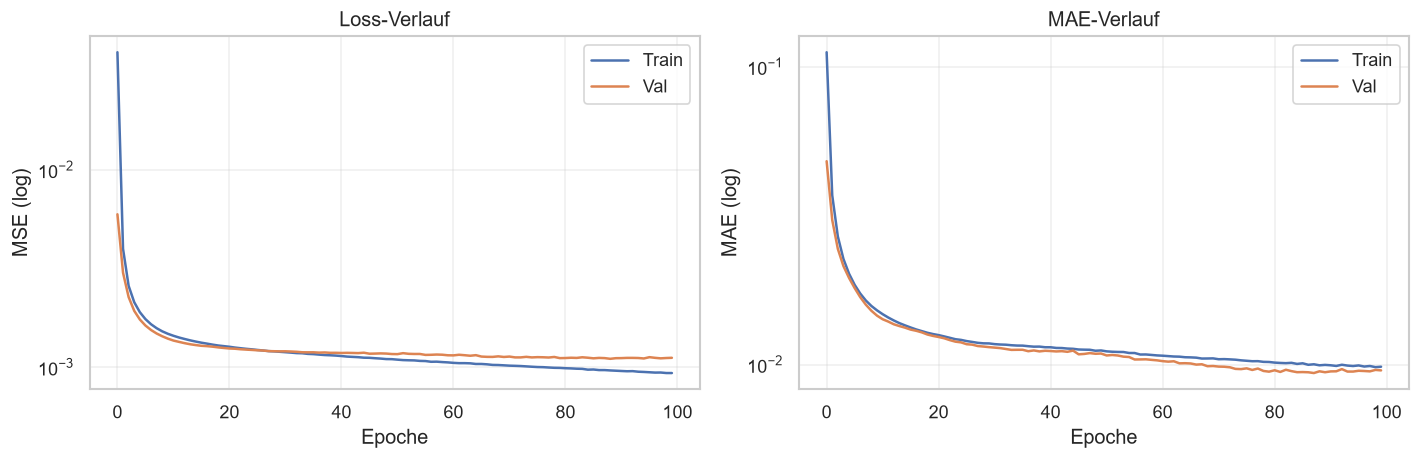
\includegraphics[width=1\linewidth]{asset/image/TomaKing_A4_Lernkurven.png}
    \caption{Lernkurven des Surrogatmodells \textit{(eigene Darstellung)}.}
    \label{fig:a4_curves}
\end{figure}

\begin{table}[H]
    \centering
    \begin{tabular}{lr}
        \toprule
        Dimension & Test-\ac{MAE} \\
        \midrule
        $x$-Position              & 0{,}00460 \\
        $y$-Position              & 0{,}00594 \\
        $v_x$                     & 0{,}00734 \\
        $v_y$                     & 0{,}00885 \\
        Winkel                    & 0{,}00443 \\
        Winkelgeschwindigkeit     & 0{,}01534 \\
        Kontakt links (binär)     & 0{,}01698 \\
        Kontakt rechts (binär)    & 0{,}01782 \\
        \bottomrule
    \end{tabular}
    \caption{Test-\ac{MAE} pro Beobachtungsdimension \textit{(eigene Darstellung)}.}
    \label{tab:a4_perdim}
\end{table}

\begin{figure}[H]
    \centering
    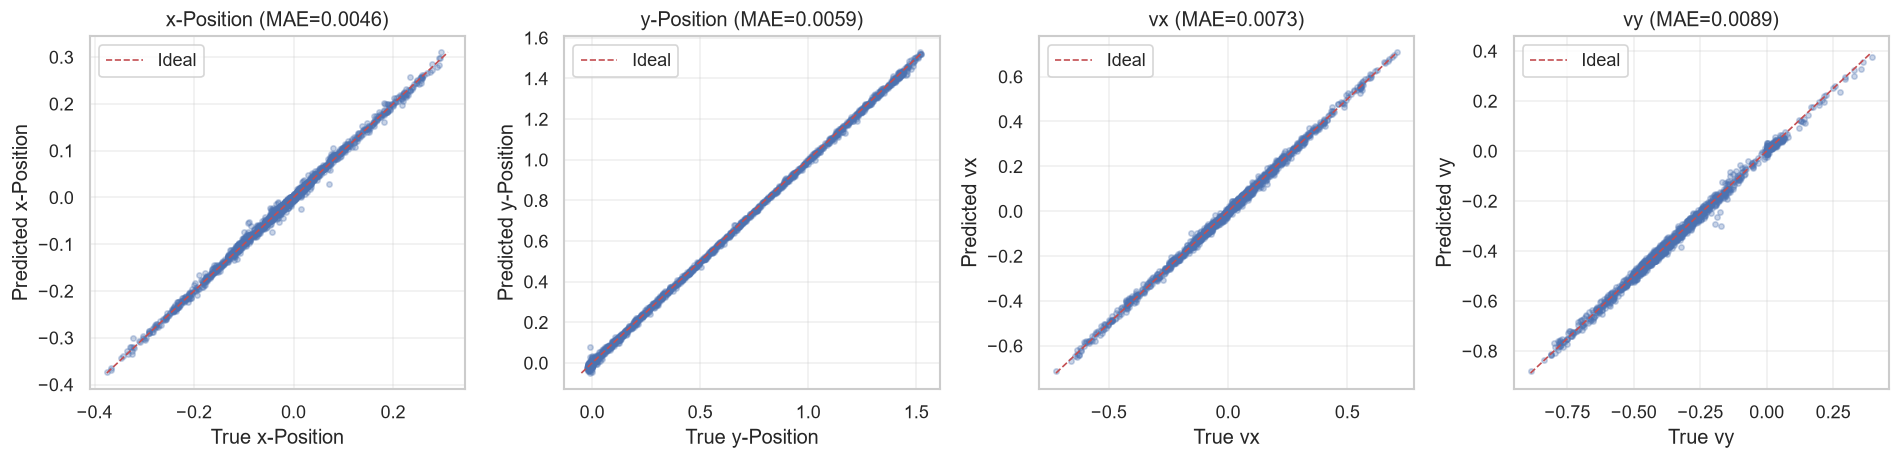
\includegraphics[width=1\linewidth]{asset/image/TomaKing_A4_Pred_vs_True.png}
    \caption{Vorhergesagte vs.\ tatsächliche Dimensionen \textit{(eigene Darstellung)}.}
    \label{fig:a4_pred}
\end{figure}

\subsection{Interpretation}

Das Modell approximiert die Zustandsübergänge sehr genau. Dies ist plausibel, da die Physik der Umgebung bis auf kleine numerische Effekte deterministisch ist. Die hohen Fehler bei den Kontakt-Flags ($\approx 0{,}017$--$0{,}018$) sind struktureller Natur: Ein Regressionsmodell kann sprunghafte 0/1-Übergänge nur annähern, für eine produktive Nutzung wäre hier eine separate binäre Klassifikation sinnvoll \cite[S.~446--448]{1}. Tabelle~\ref{tab:a4_perdim} zeigt die Fehlerverteilung über die acht Dimensionen.

% ==============================================================================
% ================================== AUFGABE 4 ================================
% ==============================================================================